\documentclass{article}
\usepackage[utf8]{inputenc}
\usepackage[letterpaper,top=1.5cm,bottom=1.5cm,left=3cm,right=3cm,marginparwidth=1.75cm]{geometry}
\usepackage{natbib}
\usepackage{graphicx}
\usepackage{tikz}
\usepackage{amsmath, amsthm, amssymb, amsfonts}
\usepackage{titlesec}
\usepackage{makecell}
\usetikzlibrary{automata,positioning}
\usetikzlibrary{arrows}
\usepackage{inconsolata}
\usepackage{chessboard}
\storechessboardstyle{5x5}{maxfield=e5, labelbottomformat=}
\usetikzlibrary{shapes}
\makeatletter
\@addtoreset{subsection}{section}
\makeatother
\def\thesection{Question \arabic{section}}
\def\thesubsection{\arabic{section}.\arabic{subsection}}
\def\thesubsubsection{\arabic{section}.\arabic{subsection}.\arabic{subsubsection}}

\title{Artificial Intelligence\\Homework no. 2}
\author{Alireza Rostami\\Student Number: 9832090}
\date{}
\begin{document}
    \maketitle
    \begin{center}
        Find the \LaTeX \ code of this masterpiece at my Github @ github.com/WellOfSorrows.
    \end{center}
    \section{}
    \subsection{}
    \qquad A special case of \textit{"Local Beam Search"} when $ k= 1 $ is called  \textit{"Hill-Climbing Search"}.
    \smallskip
    \subsection{}
    \qquad This is also \textit{hill-climbing search} since we always keep the best individual of the population, so the mutated individual only replace current individual when the fitness function improves. This is exactly  \textit{hill-climbing search}.
    \bigskip
    \section{}
    In each genetic algorithm problem, we must go through the following steps:
    \begin{enumerate}
        \item Chromosome encoding
        \item Initial population
        \item Fitness evaluation
        \item Selection
        \item Crossover
        \item Mutation
        \item Population update
        \item Iteration
    \end{enumerate}
    \medskip
    We shall go through each step one by one.
    \pagebreak
    \subsection{Encoding}
    The best way is to represent a chromosome as a string (or a list) of length $ N $ where $ N $ is the number of queens; in our case $ N=5 $.
    The value of each index shows the row of the queen in a column. For example, for the following configuration, we would have:
    \begin{table}[!ht]
    \parbox{0.45\linewidth}{
        \begin{center}
            \chessboard[style=5x5,setblack={Qa5,Qb2,Qc4,Qd3,Qe5},showmover=false]
        \end{center}
    }
    \parbox{0.35\linewidth}{
        $$
        Chromosome:       
        \begin{array}{|c|c|c|c|c|}
            \hline
            5&2&3&4&5 \\\hline
        \end{array}
        $$
    }
    \end{table}
    \subsection{Initial Population}
    Now, we initialize our population with random chromosomes. Let's take a population of 4 chromosomes as follows: 
    $$ C_1 = 
        \begin{array}{|c|c|c|c|c|}
            \hline
            5&2&3&4&5 \\\hline
        \end{array}
    $$
    $$ C_2 = 
        \begin{array}{|c|c|c|c|c|}
            \hline
            4&3&5&1&4 \\\hline
        \end{array}
    $$
    $$ C_3 = 
        \begin{array}{|c|c|c|c|c|}
            \hline
            2&1&3&2&4 \\\hline
        \end{array}
    $$
    $$ C_4 = 
        \begin{array}{|c|c|c|c|c|}
            \hline
            5&2&3&4&1 \\\hline
        \end{array}
    $$
    \subsection{Fitness Evaluation}
    Since in genetic algorithms, higher scores are better, thus we define the fitness function $ F_{total}(C)$ as number of the pairs of non-attacking queens in configuration $ C $. We also assign each queen a unique name by using its index in the chromosome as a subscription and define $ f(x_i) $ as the number of queens the queen $ x_i $ does NOT attack. So, we would attain:
    $$ F_{total}(C) = \dfrac{\sum\limits_{i=1}^{5}f(x_i)}{2} $$
    Note that we divided the sum by two because of \textit{hand-shaking lemma}. \\
    For example, for the chromosome 
    $ C_1 = 
        \begin{array}{|c|c|c|c|c|}
            \hline
            5&2&3&4&5 \\\hline
        \end{array}
    $,\quad we would have
    \begin{center}
        \chessboard[
            style=5x5,
            setblack={Qa5,Qb2,Qc4,Qd3,Qe5},
            arrow=to,
            linewidth=0.12ex,
            color=green,
            pgfstyle=straightmove,
            markmoves={a5-c4,a5-b2,a5-d3},
            shortenstart=0.1ex,
            showmover=false
        ]
        $ \Rightarrow x_1 = 3 $
    \end{center}
    \begin{center}
        \chessboard[
            style=5x5,
            setblack={Qa5,Qb2,Qc4,Qd3,Qe5},
            pgfstyle=straightmove,
            arrow=to,
            linewidth=0.125ex,
            color=green,
            pgfstyle=straightmove,
            markmoves={b2-a5,b2-c4,b2-d3},
            shortenstart=1ex,
            showmover=false
        ]
        $ \Rightarrow x_2 = 3 $
    %\end{center}
    %\begin{center}
        \chessboard[
            style=5x5,
            setblack={Qa5,Qb2,Qc4,Qd3,Qe5},
            pgfstyle=straightmove,
            arrow=to,
            linewidth=0.125ex,
            color=green,
            pgfstyle=straightmove,
            markmoves={c4-a5,c4-b2,c4-e5},
            shortenstart=1ex,
            showmover=false
        ]
        $ \Rightarrow x_3 = 3 $
    \end{center}
    \begin{center}
        \chessboard[
            style=5x5,
            setblack={Qa5,Qb2,Qc4,Qd3,Qe5},
            pgfstyle=straightmove,
            arrow=to,
            linewidth=0.125ex,
            color=green,
            pgfstyle=straightmove,
            markmoves={d3-a5,d3-b2,d3-e5},
            shortenstart=1ex,
            showmover=false
        ]
        $ \Rightarrow x_4 = 3 $
    %\end{center}
    %\begin{center}
        \chessboard[
            style=5x5,
            setblack={Qa5,Qb2,Qc4,Qd3,Qe5},
            pgfstyle=straightmove,
            arrow=to,
            linewidth=0.125ex,
            color=green,
            pgfstyle=straightmove,
            markmoves={e5-c4,e5-d3},
            shortenstart=1ex,
            showmover=false
        ]
        $ \Rightarrow x_5 = 2 $
    \end{center}
    $$ \Rightarrow F_{total}(C_1) = \frac{14}{2} = 7$$
    \\ Then, we need to compute the probability of being chosen from the fitness function. This will be needed for the selection step. First, we need to add all fitness functions of the chromosomes population. Thus, in our case, since the population is of size 4, we would have:
    $$ P(C_j) = \frac{F_{total}(C_j)}{\sum\limits_{k = 1}^{4}F_{total}(C_k)}$$
    Calculating the fitness function for other chromosomes, we would attain:
    $$
    \begin{aligned}
        F_{total}(C_2) &= 6, \\       
        F_{total}(C_3) &= 6, \\ 
        F_{total}(C_4) &= 5
    \end{aligned}
    $$
    which means that:
    $$
    \begin{aligned}
        P(C_1) &= \frac{7}{24} = 29\% \\
        P(C_2) &= \frac{6}{24} = 25\% \\       
        P(C_3) &= \frac{6}{24} = 25\% \\ 
        P(C_4) &= \frac{5}{24} = 21\%
    \end{aligned}
    $$
    \newpage
    \subsection{Selection}
    In this step, we randomly choose the two pairs to reproduce based on their probabilities. Then, selected chromosomes will act as parents and will be combined using a crossover operator to make children. For the crossover operation, we need to pick a crossover point per pair. \\
    Here we took the following chromosomes based on their probabilities:
    $$ C_1 = 
        \begin{array}{|c|c|c|c|c|}
            \hline
            5&2&3&4&5 \\\hline
        \end{array}
    $$
    $$ C_2 = 
        \begin{array}{|c|c|c|c|c|}
            \hline
            4&3&5&1&4 \\\hline
        \end{array}
    $$
    $$ C_3 = 
        \begin{array}{|c|c|c|c|c|}
            \hline
            2&1&3&2&4 \\\hline
        \end{array}
    $$ \\
    We notice that the chromosome  
    $ C_4 = 
        \begin{array}{|c|c|c|c|c|}
            \hline
            5&2&3&4&1 \\\hline
        \end{array}
    $ \quad is omitted because its probability was the least among chromosomes, making it unfit to go to the next step. Thus, the selection step would derive: \\
    \begin{center}
    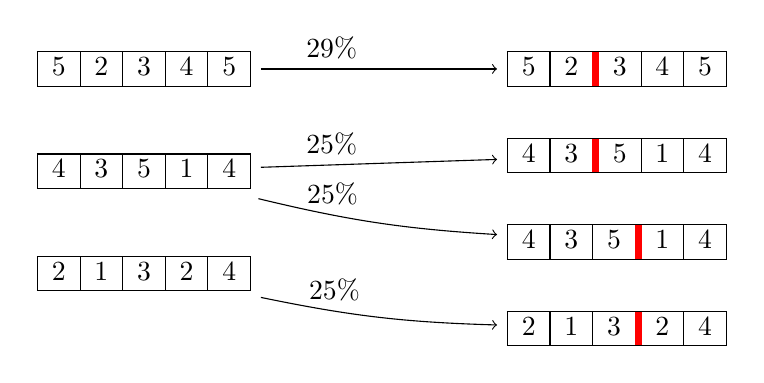
\begin{tikzpicture}
    % set up the nodes
    \node (C1) at (0,0) {
        $\begin{array}{|c|c|c|c|c|}
            \hline
            5 & 2 & 3 & 4 & 5 \\
            \hline
        \end{array}$
    };
    \node[below=0.6cm of C1] (C2) {
        $\begin{array}{|c|c|c|c|c|}
            \hline
            4&3&5&1&4 \\\hline
        \end{array}$
    };
    \node[below=0.6cm of C2] (C3) {$
        \begin{array}{|c|c|c|c|c|}
            \hline
            2&1&3&2&4 \\\hline
        \end{array}
    $};
    \node[right=3cm of C1] (nC1) { $
        \begin{array}{|c|c!{\color{red}\vrule width 2.5pt}c|c|c|}
            \hline
            5&2&3&4&5 \\\hline
        \end{array}$
    };
    \node[below=0.4cm of nC1] (nC2) { $
        \begin{array}{|c|c!{\color{red}\vrule width 2.5pt}c|c|c|}
            \hline
            4&3&5&1&4 \\\hline
        \end{array}$
    };
    \node[below=0.4cm of nC2] (nC3) { $
        \begin{array}{|c|c|c!{\color{red}\vrule width 2.5pt}c|c|}
            \hline
            4&3&5&1&4 \\\hline
        \end{array}$
    };
    \node[below=0.4cm of nC3] (nC4) { $
        \begin{array}{|c|c|c!{\color{red}\vrule width 2.5pt}c|c|}
            \hline
            2&1&3&2&4 \\\hline
        \end{array}$
    };
    % draw arrows and text between them
    \draw[->] (C1)--(nC1) node [pos=0.3, above] {$ 29\% $};
    \draw[->] (C2)--(nC2) node [pos=0.3, above] {$ 25\% $};
    \draw[->] (C2) edge [bend right = 5] node [pos=0.3, above] {$ 25\% $} (nC3);
    \draw[->] (C3) edge [bend right = 5] node [pos=0.3, above] {$ 25\% $} (nC4);
    \end{tikzpicture}
    \end{center}
    \subsection{Crossover}
    Now we use what we derived in the last step to make new children. \\
    In order to do so, a child would be created in the following way: we concatenate the first part of the child's parent with the second part of its other parent. Thus:
    \begin{center}
    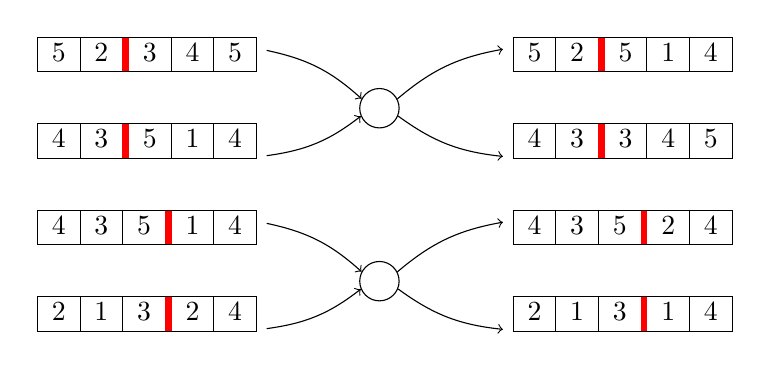
\begin{tikzpicture}
    % set up the nodes
    \node (C1) at (0,0) {$
        \begin{array}{|c|c!{\color{red}\vrule width 2.5pt}c|c|c|}
            \hline
            5&2&3&4&5 \\\hline
        \end{array}$
    };
    \node[below=0.4cm of C1] (C2) { $
        \begin{array}{|c|c!{\color{red}\vrule width 2.5pt}c|c|c|}
            \hline
            4&3&5&1&4 \\\hline
        \end{array}$
    };
    \node[below=0.4cm of C2] (C3) { $
        \begin{array}{|c|c|c!{\color{red}\vrule width 2.5pt}c|c|}
            \hline
            4&3&5&1&4 \\\hline
        \end{array}$
    };
    \node[below=0.4cm of C3] (C4) { $
        \begin{array}{|c|c|c!{\color{red}\vrule width 2.5pt}c|c|}
            \hline
            2&1&3&2&4 \\\hline
        \end{array}$
    };
    \node[right=3cm of C1] (nC1) { $
        \begin{array}{|c|c!{\color{red}\vrule width 2.5pt}c|c|c|}
            \hline
            5&2&5&1&4 \\\hline
        \end{array}$
    };
    \node[below=0.4cm of nC1] (nC2) { $
        \begin{array}{|c|c!{\color{red}\vrule width 2.5pt}c|c|c|}
            \hline
            4&3&3&4&5 \\\hline
        \end{array}$
    };
    \node[below=0.4cm of nC2] (nC3) { $
        \begin{array}{|c|c|c!{\color{red}\vrule width 2.5pt}c|c|}
            \hline
            4&3&5&2&4 \\\hline
        \end{array}$
    };
    \node[below=0.4cm of nC3] (nC4) { $
        \begin{array}{|c|c|c!{\color{red}\vrule width 2.5pt}c|c|}
            \hline
            2&1&3&1&4 \\\hline
        \end{array}$
    };
    \node[below right=0.15cm and 1.25cm of C1, draw, circle, minimum size=.5cm] (transient_1) {};
    \node[below right=0.15cm and 1.25cm of C3, draw, circle, minimum size=.5cm] (transient_2) {};
    % draw arrows and text between them
    \draw[->] (C1) edge [bend left = 15] (transient_1) node {};
    \draw[->] (C2) edge [bend right = 15] (transient_1) node {};
    \draw[->] (transient_1) edge [bend left = 15] (nC1) node {};
    \draw[->] (transient_1) edge [bend right = 15] (nC2) node {};
    \draw[->] (C3) edge [bend left = 15] (transient_2) node {};
    \draw[->] (C4) edge [bend right = 15] (transient_2) node {};
    \draw[->] (transient_2) edge [bend left = 15] (nC3) node {};
    \draw[->] (transient_2) edge [bend right = 15] (nC4) node {};
    \end{tikzpicture}
    \end{center}
    \subsection{Mutation}
     In the mutation process, we may randomly alter one or more gene values in chromosomes we attained after crossover. So in this example, a random mutation will look like the following:
    \begin{center}
    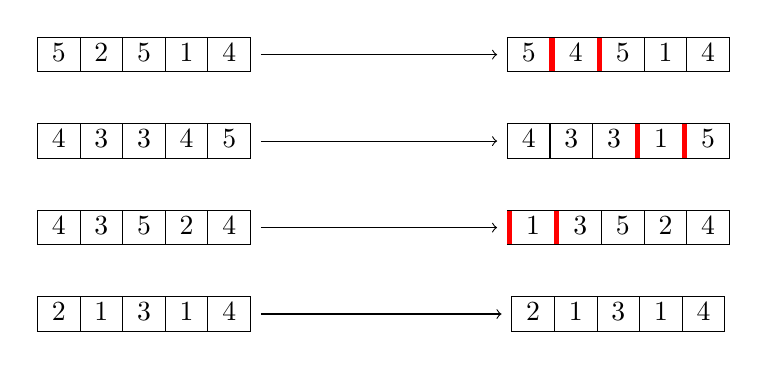
\begin{tikzpicture}
    % set up the nodes
    \node (C1) at (0,0) { $
        \begin{array}{|c|c|c|c|c|}
            \hline
            5&2&5&1&4 \\\hline
        \end{array}$
    };
    \node[below=0.4cm of C1] (C2) { $
        \begin{array}{|c|c|c|c|c|}
            \hline
            4&3&3&4&5 \\\hline
        \end{array}$
    };
    \node[below=0.4cm of C2] (C3) { $
        \begin{array}{|c|c|c|c|c|}
            \hline
            4&3&5&2&4 \\\hline
        \end{array}$
    };
    \node[below=0.4cm of C3] (C4) { $
        \begin{array}{|c|c|c|c|c|}
            \hline
            2&1&3&1&4 \\\hline
        \end{array}$
    };
    \node[right=3cm of C1] (nC1) {$
        \begin{array}{|c!{\color{red}\vrule width 2pt}c!{\color{red}\vrule width 2pt}c|c|c|}
            \hline
            5&4&5&1&4 \\\hline
        \end{array}$
    };
    \node[below=0.4cm of nC1] (nC2) { $
        \begin{array}{|c|c|c!{\color{red}\vrule width 2pt}c!{\color{red}\vrule width 2pt}c|}
            \hline
            4&3&3&1&5 \\\hline
        \end{array}$
    };
    \node[below=0.4cm of nC2] (nC3) { $
        \begin{array}{!{\color{red}\vrule width 2pt}c!{\color{red}\vrule width 2pt}c|c|c|c|}
            \hline
            1&3&5&2&4 \\\hline
        \end{array}$
    };
    \node[below=0.4cm of nC3] (nC4) { $
        \begin{array}{|c|c|c|c|c|}
            \hline
            2&1&3&1&4 \\\hline
        \end{array}$
    };
    % draw arrows and text between them
    \draw[->] (C1) edge (nC1) node {};
    \draw[->] (C2) edge (nC2) node {};
    \draw[->] (C3) edge (nC3) node {};
    \draw[->] (C4) edge (nC4) node {};
    \end{tikzpicture}
    \end{center}
    
    \subsection{Population Update}
    In this step, the chromosomes derived in the last step replaces the original population. So our population would become:
    $$ C_1 = 
        \begin{array}{|c|c|c|c|c|}
            \hline
            5&4&5&1&4 \\\hline
        \end{array}
    $$
    $$ C_2 = 
        \begin{array}{|c|c|c|c|c|}
            \hline
            4&3&3&1&5 \\\hline
        \end{array}
    $$
    $$ C_3 = 
        \begin{array}{|c|c|c|c|c|}
            \hline
            1&3&5&2&4 \\\hline
        \end{array}
    $$
    $$ C_4 = 
        \begin{array}{|c|c|c|c|c|}
            \hline
            2&1&3&1&4 \\\hline
        \end{array}
    $$
    \subsection{Iteration}
    We iterate the same procedure we illustrated (from \textit{step 3} to \textit{step 7}) until the $ F_{total} $ of one chromosome becomes:
    \[ \exists j \in \{\,1, \, 2, \, 3, \, 4\} \Rightarrow  F_{total}(C_j) = \binom{N}{2} = \binom{5}{2} = 10 \]
    This is because each queen must not attack all other queens. So, we must have a complete graph of size $ N $. The number of edges of a complete graph is $ \binom{N}{2} $.
\end{document}
